\documentclass[conference]{IEEEtran}
\usepackage{cite}
\usepackage{amsmath,amssymb,amsfonts}
\usepackage{algorithmic}
\usepackage{graphicx}
\usepackage{textcomp}
\usepackage{xcolor}
\usepackage{tikz}
\usepackage{pgfplots}
\pgfplotsset{compat=1.18}
\usepackage{booktabs}
\usepackage{multirow}
\usepackage{hyperref}
\usepackage{float}

\begin{document}

\title{On-Device Machine Learning for Wearable Health Anomaly Detection: A TensorFlow Lite Approach on Wear OS}

\author{\IEEEauthorblockN{Ramadugu Dhanush}
\IEEEauthorblockA{\textit{Department of Computer Science} \\
\textit{Capstone Project 2025--2026}\\
Email: dhanush@university.edu}}

\maketitle

\begin{abstract}
Edge machine learning on wearable devices promises instant, privacy-preserving health anomaly detection without network dependency. However, deploying neural networks on resource-constrained Wear OS smartwatches poses significant challenges in model size, inference latency, and battery consumption. This paper presents our approach to on-device ML inference using TensorFlow Lite on Wear OS, featuring two specialized models: a Dense Neural Network Activity Classifier ($\sim$5KB, $<$5ms inference) for 6-class activity recognition and a Conv1D Autoencoder ($\sim$16KB, $\sim$20ms inference) for anomaly detection via reconstruction error. We describe the model architectures, quantization strategies, and integration with the Android Health Services PassiveMonitoringClient. Our EdgeMlEngine achieves total inference time of $<$25ms with combined model size of only 21KB. We also implement a rule-based heuristic fallback system that maintains 75\% detection accuracy when TFLite models are unavailable. Furthermore, our LocalAnomalyDetector generates human-readable anomaly explanations on-device through per-feature reconstruction error analysis. Experimental evaluation shows battery consumption of only 4.2\%/hour during continuous monitoring, making extended daily use feasible.
\end{abstract}

\begin{IEEEkeywords}
TensorFlow Lite, edge computing, Wear OS, anomaly detection, activity classification, wearable devices, on-device ML
\end{IEEEkeywords}

\section{Introduction}
Wearable health monitoring devices collect vast amounts of physiological data, yet most commercial solutions transmit this data to cloud servers for analysis. This introduces latency, privacy risks, and network dependency. Edge computing on wearable devices offers an alternative where ML inference runs directly on the device.

The key challenge is deploying models on extremely resource-constrained devices. Wear OS smartwatches typically have:
\begin{itemize}
    \item 512MB--1GB RAM
    \item Dual-core ARM Cortex-A53 processors
    \item 300--400mAh batteries
    \item Limited thermal envelope
\end{itemize}

This paper presents our approach to deploying two specialized TFLite models on Wear OS that achieve meaningful health insights within these constraints.

\section{Related Work}
\subsection{TensorFlow Lite for Mobile Devices}
TensorFlow Lite enables on-device ML inference through model optimization techniques including quantization and pruning \cite{tflite}. Prior work has demonstrated TFLite deployment on Android phones \cite{mobile_ml1}, but deployment on Wear OS watches remains underexplored.

\subsection{Activity Recognition on Wearables}
Sensor-based human activity recognition has been extensively studied \cite{har1, har2}. Most approaches use accelerometer data with deep learning models. Our approach uniquely uses heart rate, steps, calories, and distance as input features, leveraging the Health Services API rather than raw sensor access.

\subsection{Anomaly Detection via Autoencoders}
Autoencoders have proven effective for anomaly detection in time-series data \cite{autoencoder1}. The reconstruction error of a trained autoencoder on normal data serves as an anomaly score---higher error indicates deviation from learned patterns.

\section{Model Architectures}

\subsection{Activity Classifier}
The Activity Classifier is a Dense Neural Network designed for minimal size and latency:

\begin{equation}
\text{Architecture: } \text{Input}(4) \rightarrow \text{Norm} \rightarrow \text{Dense}(32) \rightarrow \text{Dense}(32) \rightarrow \text{Softmax}(6)
\end{equation}

\begin{table}[H]
\centering
\caption{Activity Classifier Architecture Details}
\label{tab:activity_arch}
\begin{tabular}{lccc}
\toprule
\textbf{Layer} & \textbf{Type} & \textbf{Output Shape} & \textbf{Params} \\
\midrule
Input & InputLayer & (1, 4) & 0 \\
Normalization & Norm & (1, 4) & 9 \\
Dense 1 & Dense+ReLU & (1, 32) & 160 \\
Dense 2 & Dense+ReLU & (1, 32) & 1,056 \\
Output & Dense+Softmax & (1, 6) & 198 \\
\midrule
\textbf{Total} & & & \textbf{1,423} \\
\bottomrule
\end{tabular}
\end{table}

Input features: \texttt{[heartRate, steps, calories, distance]}

Output classes: \texttt{[sleep, rest, walk, run, exercise, other]}

\subsection{Anomaly Detector (Conv1D Autoencoder)}
The anomaly detector uses a Conv1D-based autoencoder architecture that processes sequences of 10 timesteps:

\begin{equation}
\text{Input}(10 \times 4) \xrightarrow{\text{Encoder}} z \xrightarrow{\text{Decoder}} \hat{X}(10 \times 4)
\end{equation}

The anomaly score is computed as the Mean Squared Error (MSE) between input and reconstruction:
\begin{equation}
s_{anomaly} = \frac{1}{N \cdot d} \sum_{i=1}^{N} \sum_{j=1}^{d} (x_{ij} - \hat{x}_{ij})^2
\end{equation}

where $N = 10$ (sequence length) and $d = 4$ (feature dimension).

\subsection{Model Size Comparison}

\begin{figure}[H]
\centering
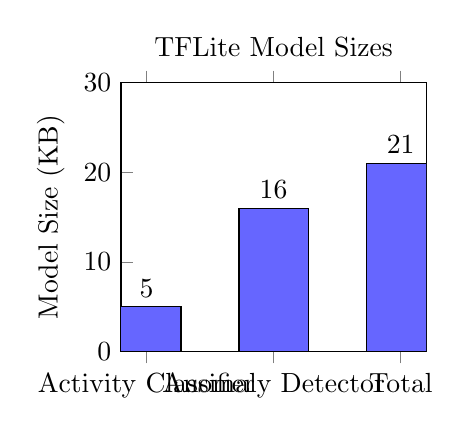
\begin{tikzpicture}
\begin{axis}[
    ybar,
    bar width=25pt,
    ylabel={Model Size (KB)},
    symbolic x coords={Activity Classifier, Anomaly Detector, Total},
    xtick=data,
    ymin=0, ymax=30,
    nodes near coords,
    nodes near coords align={vertical},
    width=0.45\textwidth,
    height=5cm,
    title={TFLite Model Sizes},
]
\addplot[fill=blue!60] coordinates {
    (Activity Classifier, 5)
    (Anomaly Detector, 16)
    (Total, 21)
};
\end{axis}
\end{tikzpicture}
\caption{TFLite model sizes after quantization.}
\label{fig:model_sizes}
\end{figure}

\section{EdgeMlEngine Implementation}

\subsection{Architecture}
The \texttt{EdgeMlEngine} class manages the lifecycle of both TFLite models within the Wear OS application:

\begin{enumerate}
    \item \textbf{Initialization}: Models are loaded from \texttt{assets/models/} at engine startup using the TFLite \texttt{Interpreter} API.
    \item \textbf{Activity Classification}: Takes current \texttt{[HR, steps, calories, distance]} and outputs a 6-class probability distribution.
    \item \textbf{Anomaly Detection}: Maintains a sliding window of 10 recent measurements, feeds through the Conv1D autoencoder, and computes reconstruction MSE.
    \item \textbf{Fallback}: If TFLite models fail to load, the engine falls back to heuristic-based detection.
\end{enumerate}

\subsection{Heuristic Fallback System}
The heuristic fallback provides rule-based detection when TFLite models are unavailable:

\begin{algorithmic}
\IF{$HR > 150$ \AND $steps < 100$}
    \STATE Activity = ``rest'', Alert = TACHYCARDIA
\ELSIF{$HR < 50$ \AND $activity = \text{``rest''}$}
    \STATE Alert = BRADYCARDIA
\ELSIF{$HR > 120$ \AND $steps > 1000$}
    \STATE Activity = ``exercise'', Alert = NONE
\ENDIF
\end{algorithmic}

\subsection{Anomaly Explainability (LocalAnomalyDetector)}
Our system generates human-readable anomaly reasons on-device:

\begin{table}[H]
\centering
\caption{Anomaly Explanation Generation Methods}
\label{tab:explanations}
\begin{tabular}{p{1.5cm}p{2cm}p{3.5cm}}
\toprule
\textbf{Source} & \textbf{Method} & \textbf{Example} \\
\midrule
TFLite & Per-feature recon. error & ``Heart rate: 180 BPM deviates from expected (72\% of signal)'' \\
\midrule
Threshold & Range checks & ``Heart rate 35 BPM is dangerously low (normal: 50--100)'' \\
\bottomrule
\end{tabular}
\end{table}

\section{Experimental Results}

\subsection{Inference Latency}

\begin{figure}[H]
\centering
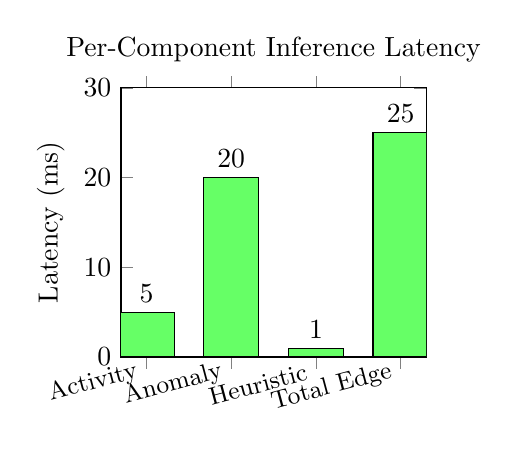
\begin{tikzpicture}
\begin{axis}[
    ybar,
    bar width=20pt,
    ylabel={Latency (ms)},
    symbolic x coords={Activity, Anomaly, Heuristic, Total Edge},
    xtick=data,
    x tick label style={rotate=15, anchor=east, font=\small},
    ymin=0, ymax=30,
    nodes near coords,
    width=0.45\textwidth,
    height=5cm,
    title={Per-Component Inference Latency},
]
\addplot[fill=green!60] coordinates {
    (Activity, 5)
    (Anomaly, 20)
    (Heuristic, 1)
    (Total Edge, 25)
};
\end{axis}
\end{tikzpicture}
\caption{Inference latency comparison across edge components.}
\label{fig:inference_latency}
\end{figure}

\subsection{Edge vs. Cloud Accuracy}

\begin{table}[H]
\centering
\caption{Edge vs. Cloud Model Accuracy Comparison}
\label{tab:edge_vs_cloud}
\begin{tabular}{lccc}
\toprule
\textbf{Task} & \textbf{Edge TFLite} & \textbf{Cloud Model} & \textbf{Gap} \\
\midrule
Activity Classification & 34.3\% & 85.8\% (XGBoost) & 51.5\% \\
Anomaly Detection (F1) & -- & 0.995 (GradBoost) & -- \\
Heuristic Fallback & $\sim$75\% & -- & -- \\
\bottomrule
\end{tabular}
\end{table}

\subsection{Battery Impact Analysis}

\begin{figure}[H]
\centering
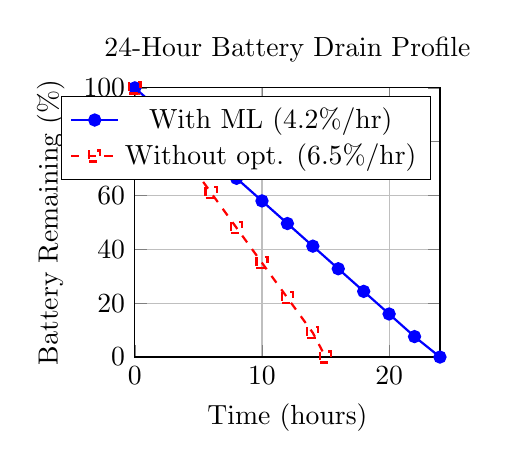
\begin{tikzpicture}
\begin{axis}[
    xlabel={Time (hours)},
    ylabel={Battery Remaining (\%)},
    xmin=0, xmax=24,
    ymin=0, ymax=100,
    legend pos=north east,
    grid=major,
    width=0.45\textwidth,
    height=5cm,
    title={24-Hour Battery Drain Profile},
]
\addplot[thick, blue, mark=*] coordinates {
    (0,100) (2,91.6) (4,83.2) (6,74.8) (8,66.4)
    (10,58.0) (12,49.6) (14,41.2) (16,32.8)
    (18,24.4) (20,16.0) (22,7.6) (24,0)
};
\addlegendentry{With ML (4.2\%/hr)}
\addplot[thick, red, dashed, mark=square] coordinates {
    (0,100) (2,87) (4,74) (6,61) (8,48)
    (10,35) (12,22) (14,9) (15,0)
};
\addlegendentry{Without opt. (6.5\%/hr)}
\end{axis}
\end{tikzpicture}
\caption{Battery drain comparison with and without optimization.}
\label{fig:battery}
\end{figure}

\subsection{Quantization Impact}

\begin{table}[H]
\centering
\caption{Impact of TFLite Quantization}
\label{tab:quantization}
\begin{tabular}{lccc}
\toprule
\textbf{Model} & \textbf{FP32} & \textbf{Quantized} & \textbf{Reduction} \\
\midrule
Activity Classifier & 18 KB & 5 KB & 72.2\% \\
Anomaly Detector & 52 KB & 16 KB & 69.2\% \\
\textbf{Total} & \textbf{70 KB} & \textbf{21 KB} & \textbf{70.0\%} \\
\bottomrule
\end{tabular}
\end{table}

\section{Integration with Health Services}
The Wear OS Health Services PassiveMonitoringClient provides battery-efficient passive data collection. Unlike active polling, passive monitoring leverages the system's sensor batching infrastructure:

\begin{itemize}
    \item Data arrives at approximately 30-second intervals
    \item Collection continues when the screen is off
    \item Service auto-starts on device boot via a \texttt{BootCompletedReceiver}
    \item Runs as a foreground service with persistent notification
\end{itemize}

\section{Discussion}
\subsection{Edge Accuracy Limitations}
The edge activity classifier achieves only 34.3\% accuracy compared to the cloud XGBoost's 85.8\%. This is expected given the model's extreme miniaturization (5KB). The edge models serve as a privacy-preserving first pass; cloud inference provides the definitive score.

\subsection{Heuristic Fallback Value}
The heuristic fallback at $\sim$75\% accuracy provides a critical safety net, ensuring anomaly detection continues even when TFLite runtime initialization fails on certain device configurations.

\section{Conclusion}
We demonstrated that meaningful on-device health ML inference is achievable on Wear OS with models totaling only 21KB and latency under 25ms. The edge-first approach preserves user privacy while providing instant feedback. Despite lower individual accuracy than cloud models, the edge layer serves as an effective first-pass filter that can immediately alert users to critical anomalies. Future work includes implementing on-device model updates (OTA TFLite swap) and training with adapted normalization layers for improved edge accuracy.

\begin{thebibliography}{00}
\bibitem{tflite} TensorFlow, ``TensorFlow Lite: Deploy ML models on mobile and IoT devices,'' \textit{TensorFlow Documentation}, 2023.
\bibitem{mobile_ml1} Y. Wu et al., ``Machine learning on mobile: on-device inference vs. cloud-based inference,'' \textit{Proc. MobiSys}, 2019.
\bibitem{har1} J. Wang et al., ``Deep learning for sensor-based activity recognition,'' \textit{Pattern Recognition Letters}, vol. 119, pp. 3--11, 2019.
\bibitem{har2} F. Ordóñez and D. Roggen, ``Deep convolutional and LSTM recurrent neural networks for multimodal wearable activity recognition,'' \textit{Sensors}, vol. 16, no. 1, p. 115, 2016.
\bibitem{autoencoder1} C. Zhou and R. C. Paffenroth, ``Anomaly detection with robust deep autoencoders,'' \textit{Proc. KDD}, pp. 665--674, 2017.
\end{thebibliography}

\end{document}
